\documentclass[10pt,a4paper]{article}
\usepackage[utf8]{inputenc}
\usepackage[T1]{fontenc}
\usepackage{amsmath}
\usepackage{amssymb}
\usepackage{graphicx}


\usepackage{hyperref}
%\usepackage{url}
\usepackage{xspace}
\usepackage{float}
\restylefloat{figure}

\usepackage{rotating}
\usepackage{array}
\newcolumntype{L}{>{\centering\arraybackslash}m{4.cm}}
\newcolumntype{I}{>{\centering\arraybackslash}m{2.25cm}}
\newcolumntype{S}{>{\centering\arraybackslash}m{1cm}}

\usepackage[table]{xcolor}    % loads also »colortbl«
\definecolor{keywordsColor}{rgb}{0.000000, 0.000000, 0.635294}
\definecolor{commentsColor}{rgb}{0.497495, 0.497587, 0.497464}
\definecolor{stringColor}{rgb}{0.558215, 0.000000, 0.135316}


\usepackage{tikz}
\usepackage{xcolor}
\definecolor{corn}{rgb}{0.98, 0.93, 0.36}
\definecolor{emerald}{rgb}{0.31, 0.78, 0.47}

\usetikzlibrary{positioning,patterns,arrows,decorations.markings,decorations.pathreplacing,shapes,shapes.misc}


\def\non{\nonumber}
\def\p{\partial}
\def\o{\over}
\def\etc{\emph{etc}.\xspace}




\title{QALB LaTeX-Generated Images}
\author{Daniel Gr\"unbaum}
\begin{document}
	
\begin{figure}[t] 
	\begin{center}
		\resizebox{6.5cm}{!}{
			
			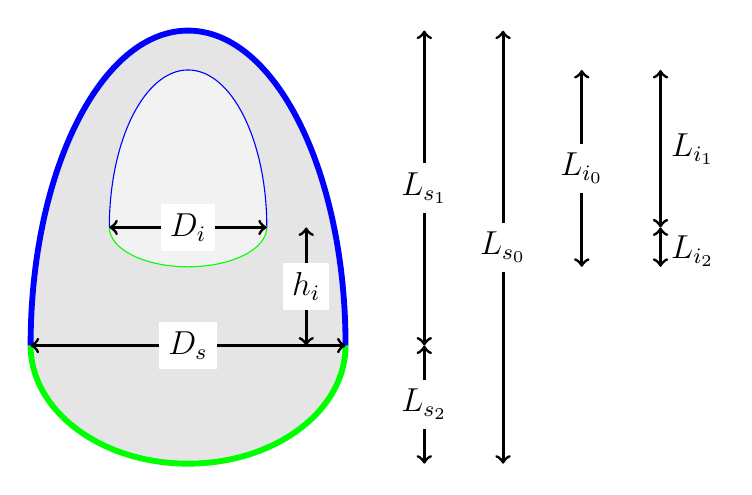
\begin{tikzpicture}
				% Outer (surface) chimera
				\filldraw[blue][fill=gray!20!white,line width=0.742mm] (2,0) arc
				[
				start angle=0,
				end angle=180,
				x radius=2cm,
				y radius =4cm
				] ;
				\filldraw[green][fill=gray!20!white,line width=0.742mm] (2,0) arc
				[
				start angle=0,
				end angle=-180,
				x radius=2cm,
				y radius =1.5cm
				] ;
				\coordinate []  (A) at (-2,0)  ;
				\coordinate []  (B) at (2,0) ;
				\coordinate []  (A1) at (3,4)  ;
				\coordinate []  (B1) at (3,-1.5) ;		
				\coordinate []  (A2) at (4,4)  ;
				\coordinate []  (B2) at (4,-1.5) ;		
				\coordinate []  (equator) at (3,0) ;
				\path[<->] (A) edge[line width=0.371mm] node[ fill=white, anchor=center, pos=0.5,font=\bfseries] {\large $D_s$} (B);
				\path[<->] (equator) edge[line width=0.371mm] node[ fill=white, anchor=center, pos=0.5,font=\bfseries] {\large $L_{s_1}$} (A1);
				\path[<->] (equator) edge[line width=0.371mm] node[ fill=white, anchor=center, pos=0.5,font=\bfseries] {\large $L_{s_2}$} (B1);
				\path[<->] (A2) edge[line width=0.371mm] node[ fill=white, anchor=center, pos=0.5,font=\bfseries] {\large $L_{s_0}$} (B2);
				\filldraw[blue][fill=gray!10!white] (1,1.5) arc
				% Inner chimera
				[
				start angle=0,
				end angle=180,
				x radius=1cm,
				y radius =2cm
				] ;
				\draw[green][fill=gray!10!white] (1,1.5) arc
				[
				start angle=0,
				end angle=-180,
				x radius=1cm,
				y radius = 0.5cm
				] ;
				\coordinate []  (A3) at (-1,1.5)  ;
				\coordinate []  (B3) at (1,1.5) ;
				\coordinate []  (A4) at (6,3.5)  ;
				\coordinate []  (B4) at (6,1) ;		
				\coordinate []  (A5) at (5,3.5)  ;
				\coordinate []  (B5) at (5,1) ;		
				\coordinate []  (equator2) at (6,1.5) ;
				\coordinate []  (h0) at (1.5,0) ;
				\coordinate []  (h1) at (1.5,1.5) ;
				\path[<->] (A3) edge[line width=0.371mm] node[ fill=white, anchor=center, pos=0.5,font=\bfseries] {\large $D_i$} (B3);
				\path[<->] (equator2) edge[line width=0.371mm] node[anchor=west, pos=0.5,font=\bfseries] {\large $L_{i_1}$} (A4);
				\path[<->] (equator2) edge[line width=0.371mm] node[anchor=west, pos=0.6,font=\bfseries] {\large $L_{i_2}$} (B4);
				\path[<->] (A5) edge[line width=0.371mm] node[ fill=white, anchor=center, pos=0.5,font=\bfseries] {\large $L_{i_0}$} (B5);
				\path[<->] (h0) edge[line width=0.371mm] node[ fill=white, anchor=center, pos=0.5,font=\bfseries] {\large $h_i$} (h1);
			\end{tikzpicture}
		}
	\end{center}
	\caption{Layout of a composite chimera, in profile view, with a constitutive chimera representing the exterior surface (parameterized by $D_s$, $L_{s_0}$, \etc) and a nested constitutive chimera representing an inclusion (parameterized by $D_i$, $L_{i_0}$, \etc). 
		$h_i$ is the height by which the equator of the inclusion chimera is elevated relative to the equator of the surface chimera (which may be negative). 
		%The schematic shows the inclusion chimera being co-axial with the surface chimera. 
		%In the numerical implementation, inclusions may be offset horizontally, as long as no chimera surfaces intersect.
	} \label{fig:chimera2}
\end{figure}
	
	
	
\end{document}